\begin{center}
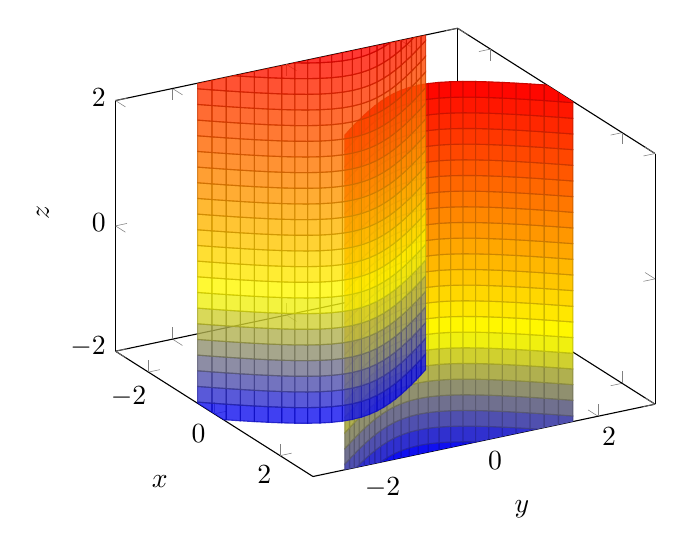
\begin{tikzpicture}
    \begin{axis}[
        view={60}{30},
        xlabel={$x$},
        ylabel={$y$},
        zlabel={$z$},
        xmin=-3, xmax=3,
        ymin=-3, ymax=3,
        zmin=-2, zmax=2,
        samples = 25
    ]

    % Hyperbolic cylinder: x^2 - z^2 = 1
    \addplot3 [
        surf, 
        domain=-2:2,    % Range for z
        domain y=-3:3,  % Range for y (hyperbola parameter)
        z buffer=sort,
        colormap/hot
    ] 
    ({sqrt(x^2 + 1)}, x, y); % Parametric equation of the hyperbolic cylinder (right branch)

    \addplot3 [
        surf, 
        domain=-2:2,    % Range for z
        domain y=-3:3,  % Range for y (hyperbola parameter)
        z buffer=sort,
        colormap/hot,
        opacity=0.8
    ] 
    ({-sqrt(x^2 + 1)}, x, y); % Parametric equation of the hyperbolic cylinder (left branch)

    \end{axis}
\end{tikzpicture}
\end{center}